% last updated in April 2002 by Antje Endemann
% Based on CVPR 07 and LNCS, with modifications by DAF, AZ and elle, 2008 and AA, 2010, and CC, 2011

\documentclass[runningheads]{llncs}
\usepackage{graphicx}
\usepackage[font=small]{caption}
\usepackage{subcaption}
\captionsetup{compatibility=false}
\usepackage{amsmath,amssymb} % define this before the line numbering.
\usepackage{ruler}
\usepackage{color}
\usepackage{url}
\usepackage[width=122mm,left=12mm,paperwidth=146mm,height=193mm,top=12mm,paperheight=217mm]{geometry}
\usepackage{multirow}

\begin{document}
% \renewcommand\thelinenumber{\color[rgb]{0.2,0.5,0.8}\normalfont\sffamily\scriptsize\arabic{linenumber}\color[rgb]{0,0,0}}
% \renewcommand\makeLineNumber {\hss\thelinenumber\ \hspace{6mm} \rlap{\hskip\textwidth\ \hspace{6.5mm}\thelinenumber}}
% \linenumbers \

\pagestyle{headings}
\mainmatter
\def\ECCV14SubNumber{150}  % Insert your submission number here

\title{Design of Blur Invariant Fiducial for Low Cost Quadcopter} % Replace
% with your title

\titlerunning{ECCV-14 submission ID \ECCV14SubNumber}

\authorrunning{ECCV-14 submission ID \ECCV14SubNumber}

\author{Anonymous ECCV submission}
\institute{Paper ID \ECCV14SubNumber}

\maketitle

\begin{abstract}
Fiducial markers are commonly used to track an object in an unknown environment
and finds use in various applications in Virtual Reality, Medical imaging,
Surveys, etc. The performance of popular fiducials is satisfactory when there is
little motion or no motion in the device obtaining the imagery. But when there
is continuous and swift motion, as in the case of low cost quadcopters,
performance of these fiducials degrade significantly due to motion blur.
Inspired from Circular Data Matrix\cite{NaimarkF02}, we have designed a fiducial
that may be thought of as a binary code. It contains concentric white rings of
equal widths on a black background with a blurred border. Our fiducial detection
algorithm is based on the fact that there is no blur in the direction
perpendicular to the direction of the motion. The algorithm finds this
direction in a simple but accurate way. Then, we find ``signature'' of our
fiducial along this direction and further classify it to find the actual code
embedded in the fiducial. We will show through experimental validation that our
fiducial works better than popular fiducials such as ARTag under signifacant motion blur.

\keywords{Fiducials, Tracking, Blur Invariant}
\end{abstract}

\section{Introduction}
A fiducial marker or simply a fiducial is an synthetic object placed in the
scene, which can provide additional information about the environment. Sometimes
naturally available features in a scene may be used as replacement to fiducials.
But, natural features may not be available always and quality cannot be
guranteed in every scene. So, results are not satisfactory in uncontrolled
environment and hence use of such features is limited. Artificial fiducials are
widely used in Augmented Reality(AR)\cite{Zhang:2002}\cite{Dorfmuller99}
applications, vision based navigation of robots\cite{Davison:2007} etc.

Recently, use of Unmanned Aerial Vehicles(UAV) such as quadcopters is increased
in various tracking activities (e.g. aerial surveillance, search and rescue
operations etc.).Low cost quadcopters such as AR Drone are very unstable which
causes non-uniform motion resulting lot of motion blur in captured images.
Also, as image transfer is done through wireless media using User Datagram
Protocol (UDP), there is possibility of missing intermediate frames . It
results in lower frame rate (around 15 frames per second (FPS)) instead of
normal rate of 30 FPS. This frequent dropping of frames may cause drastic
change in position of object in successive frames. Thus, performance of
traditional tracking methods is not satisfactory for tracking through
quadcopters. Our aim is to design a fiducial which we will be able to track
under significant amount of motion blur and is robust in terms of drastic
change in its position in successive frames.

We observed that blur in a single frame captured through quadcopter is linear.
There is no blur in the direction perpendicular to the direction of motion. We
tried to design a fiducial whose ``signature'' remains intact in any direction.

\begin{figure}
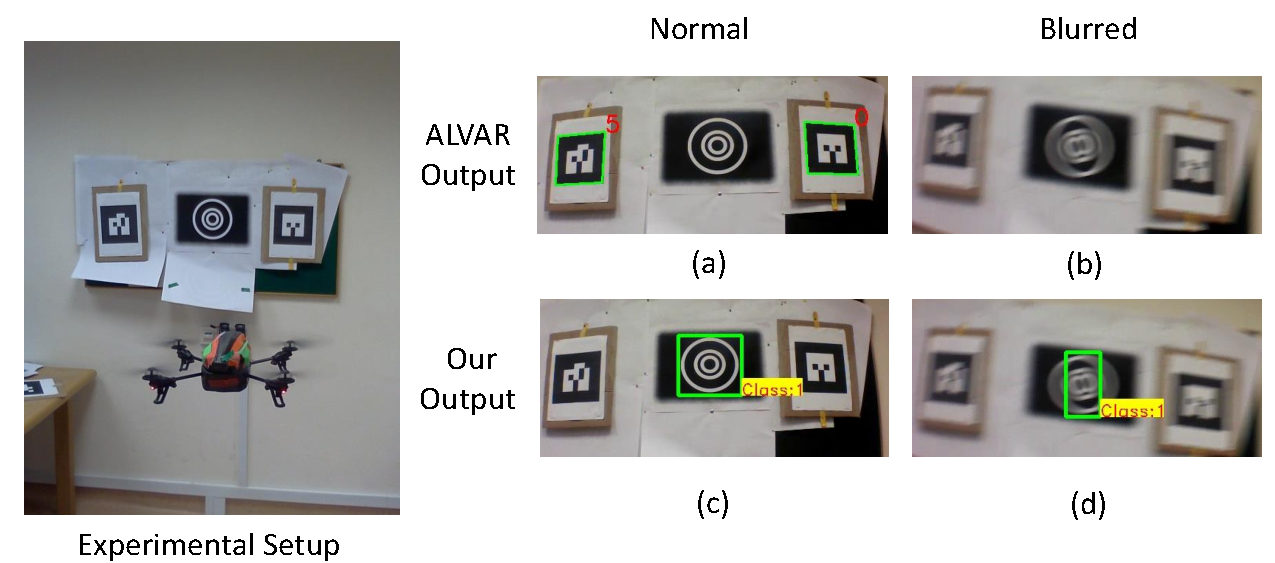
\includegraphics[width=\linewidth]{teaser.pdf}
\caption{Figure showing experimental setup and comparison of
output of ALVAR\cite{alvar} (for detecting ARTag) versus output of our
algorithm, in normal and blurred scene}
\end{figure}
 
\section{Related Work}
Our problem may be classified broadly in two areas; fiducial markers and
tracking. So, we will briefly discuss work done in both areas.
\begin{figure}
 \begin{subfigure}[b]{0.19\textwidth}
  \centering
  
\includegraphics[width=\linewidth]{intersense.jpg}
  Intersense\cite{NaimarkF02}  
 \end{subfigure}
 \begin{subfigure}[b]{0.19\textwidth}  
 \centering 
  
\includegraphics[width=\linewidth]{pattKanji.pdf}
  ARToolkit\cite{ARToolkit02}  
 \end{subfigure}
 \begin{subfigure}[b]{0.19\textwidth}
  \centering
  
\includegraphics[width=\linewidth]{ARtag.jpg}
  ARTag\cite{Fiala05}
 \end{subfigure} 
 \begin{subfigure}[b]{0.19\textwidth}
  \centering
  
\includegraphics[width=\linewidth]{pifiducial.png}
  Pi-Tag\cite{Pitag13}  
 \end{subfigure}
 \begin{subfigure}[b]{0.19\textwidth}
  \centering
  
\includegraphics[width=\linewidth]{newconcentric_01.pdf}  
  Our Fiducial  
 \end{subfigure}
 \caption{Various Fiducial Marker Designs}
 \label{fig:previous_work}  
\end{figure}
 
The ARToolkit \cite{ARToolkit02} \cite{kato-artoolkit} is well known toolkit in
Augmented Reality system, widely used to find pose of the object on which it is
placed.  Fiala et al. \cite{Fiala05} developed fiducial named, ARTag, bi-tonal
system containing 2002 planar markers, each consisting of a square border and
an interior region filled with a 6x6 grid of black or white cells. It proved to
be more efficient than \cite{ARToolkit02} in terms of marker recognition rate
as well as the number of different patterns which can be created.  

Concentric Rings are reportedly used first by Gatrell et al.\cite{concentric}
for monocular pose estimation as well as object identification in space. Cho et al.
\cite{Cho:2001}\cite{Cho97fastcolor} have used multi color rings in wide area
tracking in large scale applications. In \cite{NaimarkF02}, Naimark et al.
have developed ``Circular Data Matrix Fiducial System'', for wide area tracking.

Zhang el. al.\cite{Zhang:2002} and Claus et al. \cite{ClausF04} have done
quite comprehensive comparative study of various fiducial marker systems with
respect to processing time, recognition rate and accuracy with
respect to viewing angle and distance.

Bergamasco et al. \cite{runetag11} developed RUNE-Tag, fiducial marker
system which works under large amount of occlusion. Bergamasco et al. also 
designed Pi-Tag \cite{Pitag13}, marker design based on projective
invariants.

The main hurdle in detection of current fiducials is, the detecton of features;
lines in \cite{ARToolkit02}, corners in \cite{Fiala05} while ellipses in
\cite{Cho:2001}, \cite{Cho97fastcolor}, \cite{runetag11} and \cite{Pitag13}.
Such features are very difficult to detect accurately under significant motion
blur. So, under blur, recognition rate of these fiducials is very low. 

Fiducial detection in video may be considered as tracking problem where tracked
object is fiducial itself. Visual tracking plays an important role in
surveillance, robotics, human computer interaction, and medical
imaging\cite{Yilmaz:2006}. Yilmaz et al.\cite{Yilmaz:2006} have done survey of
various tracking methods. Most tracking methods
( \cite{Ross:2008} \cite{Wu:2009} \cite{Perez02} \cite{Mei:2009} ) assume image
sequence to be blur free. But in reality, motion blur is inherent part of most
of the videos. Wu et al.\cite{Wu:2011} have developed BLUr-driven Tracker (BLUT)
framework for tracking motion-blurred targets. BLUT is based on the observation
that although motion blurs degrade the visual features of the target, they, at
thde same time, provide useful cues about the movements to help tracking.
 
BLUT framework successfully tracks blurred target when there is uniform motion
and the position of tracked object does not change drastically in successive
frames. But in our case, due to frequntly dropping of intermediate frame, this
criterion may not be satisfied.
 
\section{Design of Fiducial}

\begin{figure}
\centering
  
\includegraphics[width=.22\linewidth]{newconcentric_00.pdf}  
  
\includegraphics[width=.22\linewidth]{newconcentric_01.pdf}
  
\includegraphics[width=.22\linewidth]{newconcentric_10.pdf}
  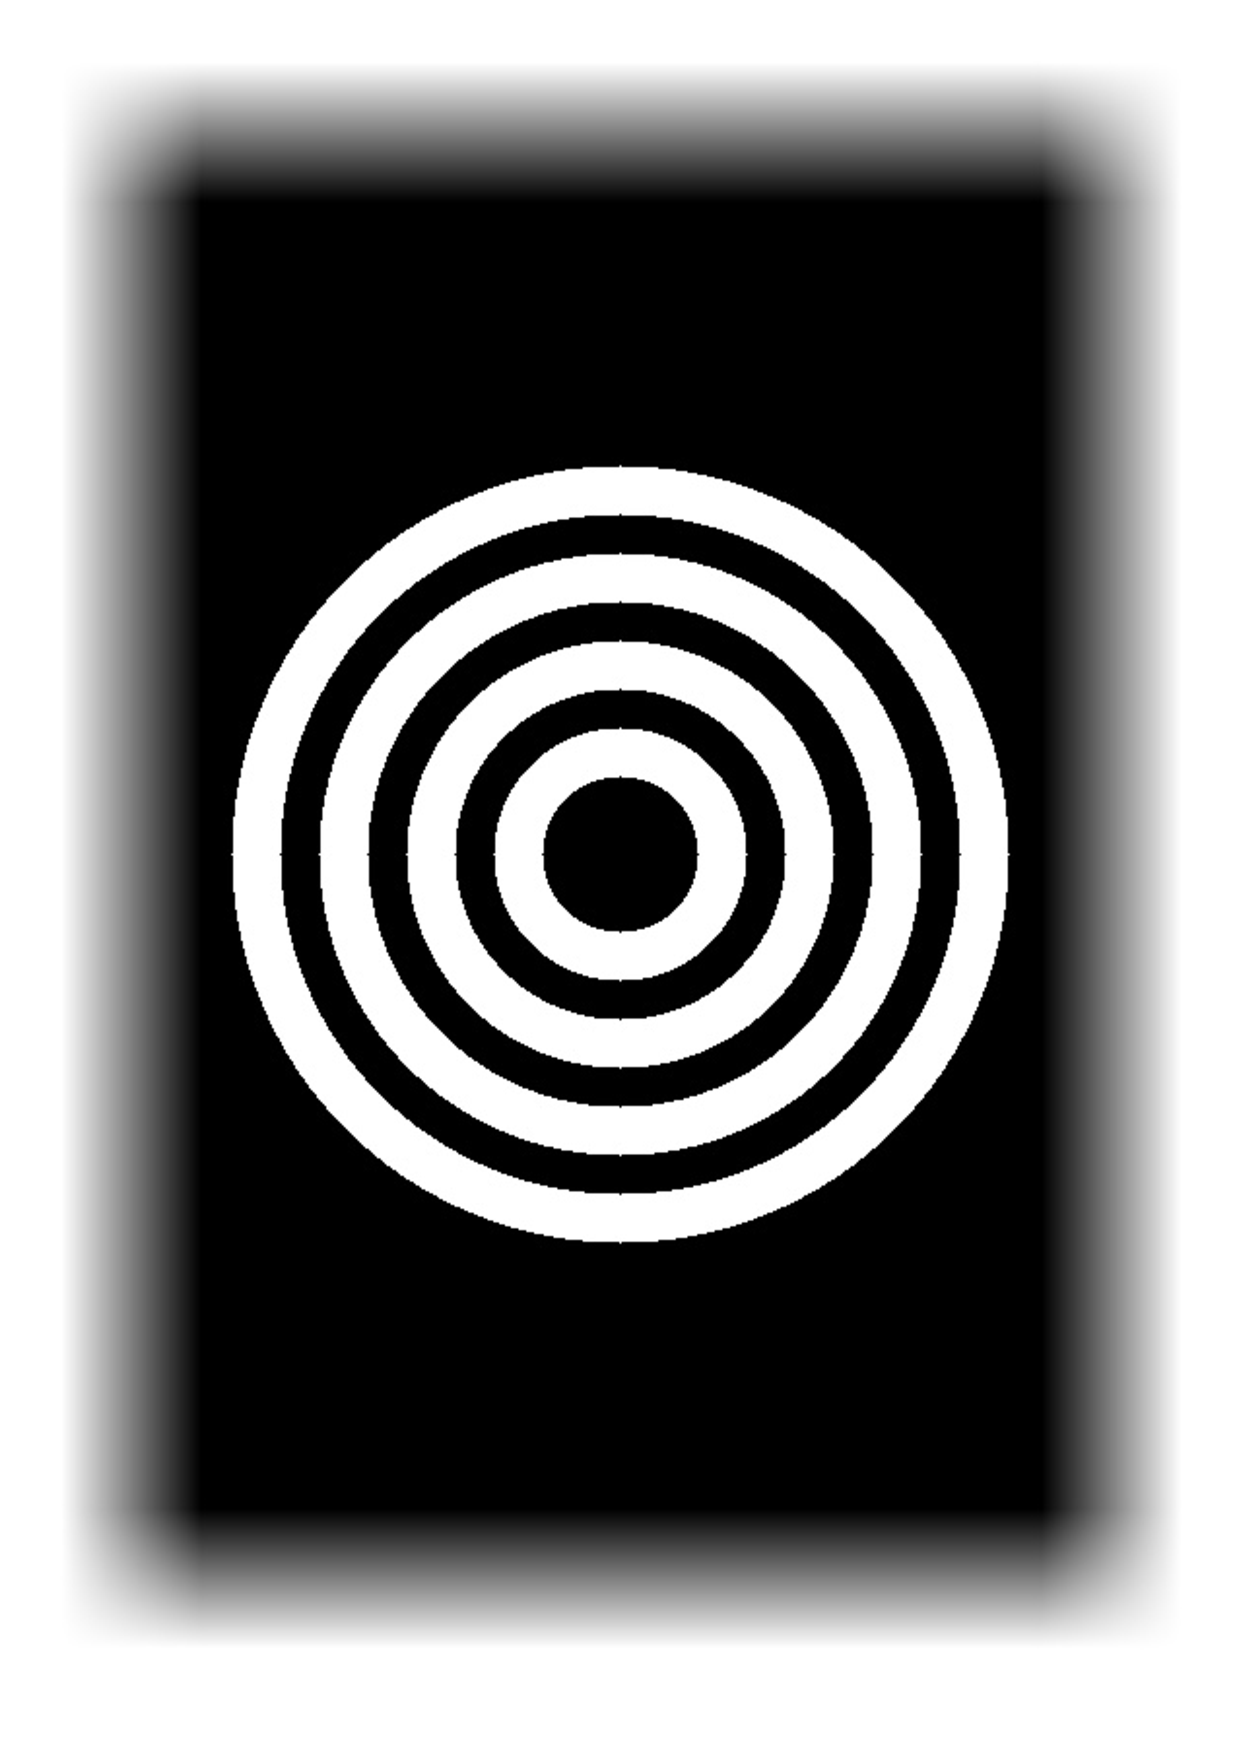
\includegraphics[width=.22\linewidth]{newconcentric_11.pdf}
  \caption{Two bit binary coded Fiducials (from left to right: Binary Code 00,
  Binary Code 01, Binary Code 10, Binary Code 11)}
  \label{fig:fiducials}
\end{figure}

Inspired from Circular Data Matrix\cite{NaimarkF02} we have designed a fiducial
that may be thought of as a binary code.  It contains concentric white rings of
equal widths on a black background with a blurred border. The outermost and
innermost rings represent the start and end of the code and is embedded in the
fiducial; these are not considered part of the code itself. The binary code is
represented by the presence (or absence) of rings between ``marker'' rings.

Depending on which ring is present or absent, the resulting binary code will
change. The number of different patterns depends on the number of bits in the
binary code. For example, if the binary code has three bits, there will be a
maximum of three rings between``marker'' rings and we end up with eight
different patterns. Fig. \ref{fig:fiducials} shows two bit binary coded
fiducials.

\section{Fiducial Detection Algorithm}
\begin{figure}
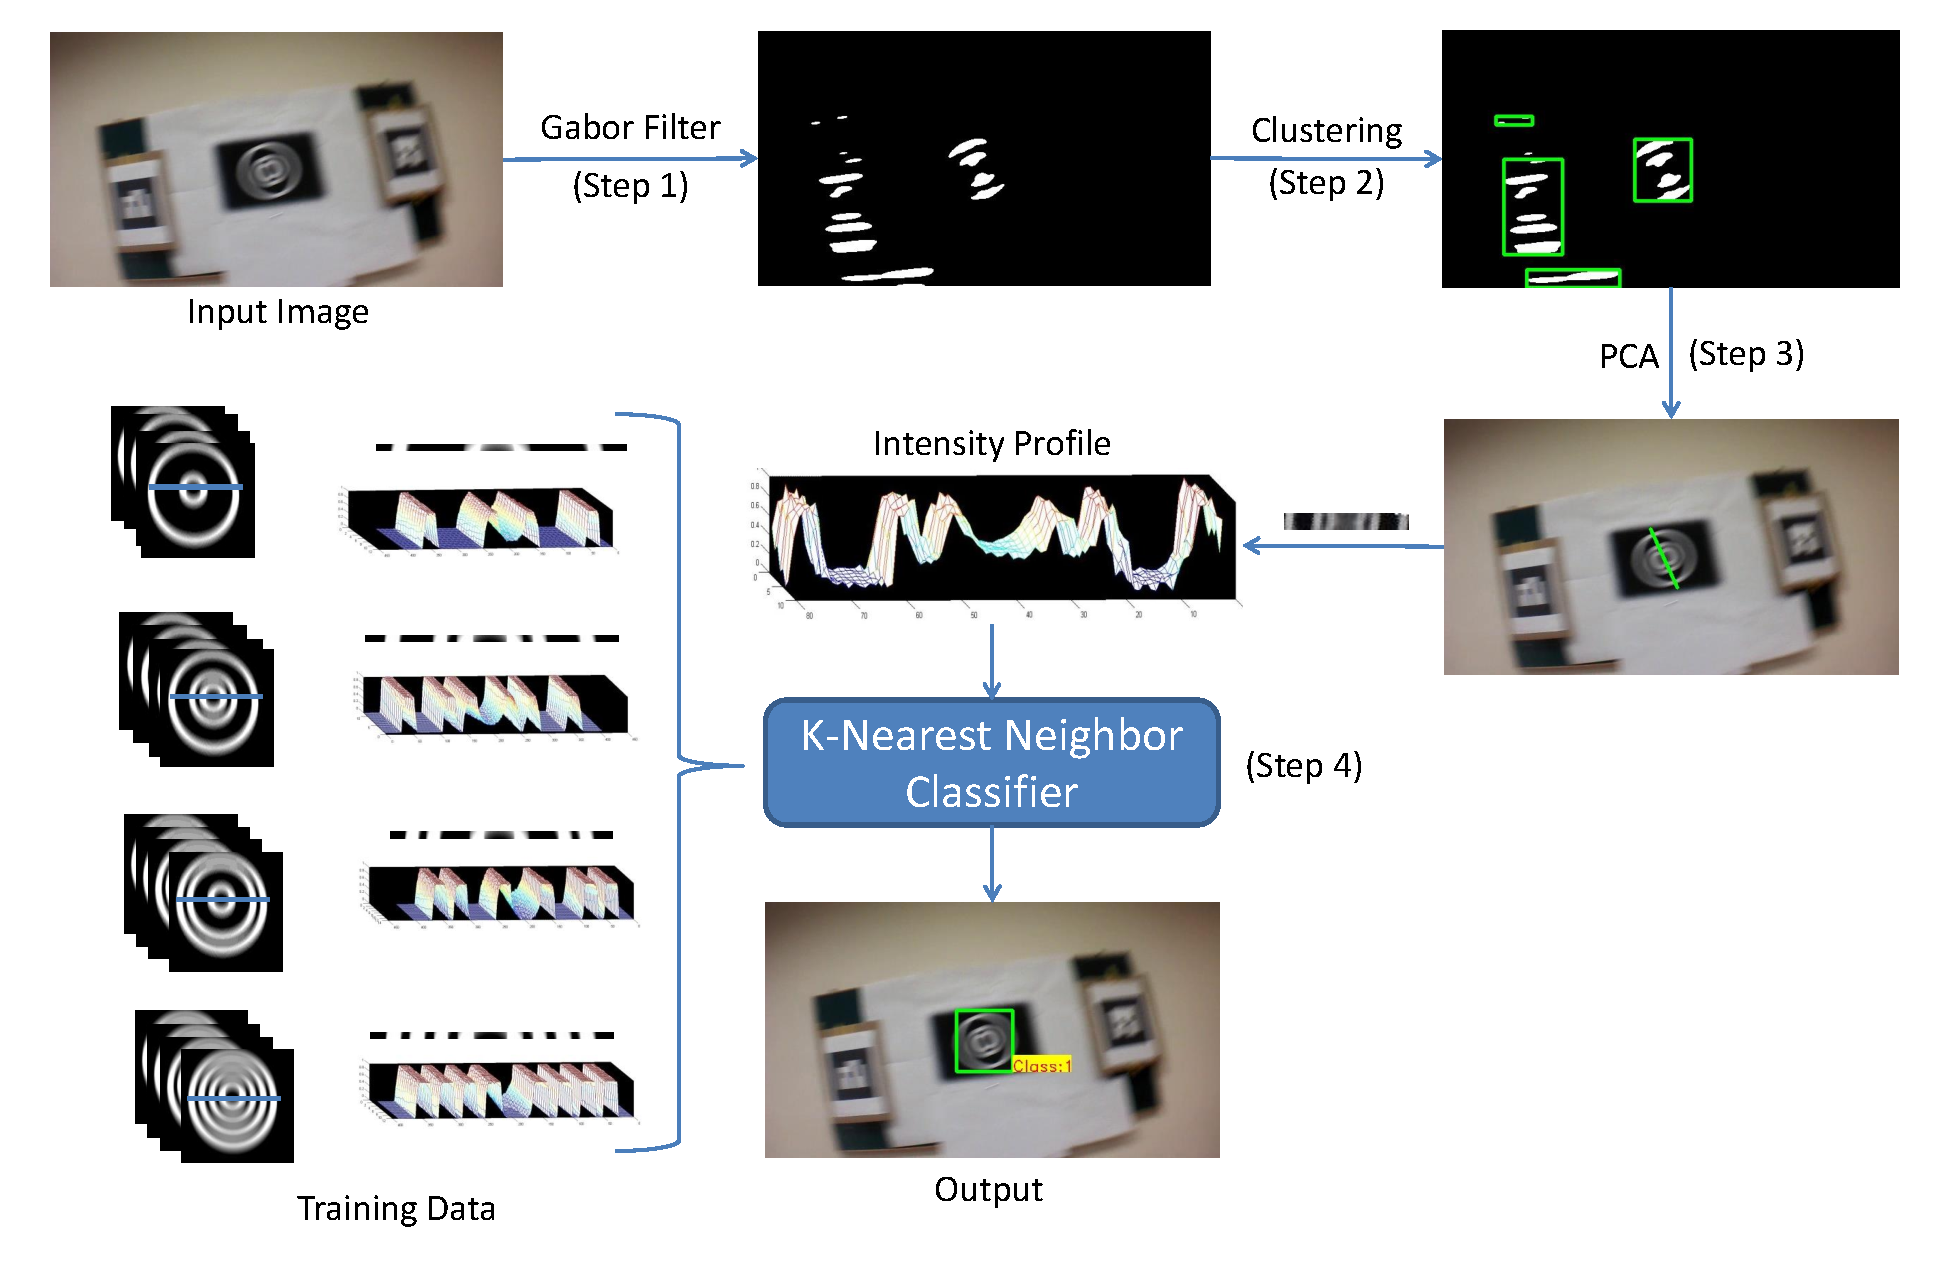
\includegraphics[width=\linewidth]{overall_flow.pdf}
\caption{Overall Workflow}
\end{figure}
Our fiducial detection strategy is different from \cite{NaimarkF02} and works
under significant amount of blur. Our algorithm is based on the fact that there
is no blur in the direction perpendicular to the direction of the motion.
Overall flow of fiducial detection algorithm can be summarised as follows:
\begin{itemize}
  \item Apply Gabor Filter on input image
  \item Find Connected components in Gabor output
  \item Cluster the connected components in bounding box
  \item Detect code in the bounding box
  \begin{itemize}
    \item Run PCA on Gabor output in bounding box
    \item Find intensity profile along first principal component passing through
    centroid
    \item If there are less than four black to white transitions in the
    intensity profile, ignore the bouding box
    \item Otherwise, classify the detected code by the classifer trained on
    standards.
  \end{itemize}
\end{itemize}

\textbf{Gabor Filter}: A 2D Gabor filter is a Gaussian kernel function modulated
by a sinusoidal plane wave. It is used to find high gradient patches from the
image. In our case, it will detect blur invariant sections of the fiducials. We
have applied Gabor filter for eight different orientations ($\theta = 0, 45,
90, 135, 180, 225, 270, 315$) and then calculated L2 norm of all outputs.

\textbf{Clustering}: Connected components are found from the Gabor output. 
These connected components are then clustered in hierarchical fashion, to find
the group of closely positioned patches.

\textbf{PCA}: Principal Component Analysis is done on the clustered Gabor
output. Along first principal component, intensity profile in the original image
is found. Number of transitions in the intensity profile will give us the
number of rings.

\textbf{Classification}: Each synthetic fiducial pattern is blurred along 36
orientations (0, 10, 20, \ldots , 350) and intensity profile along first
principal component from every output is taken as training data for that fiducial pattern.
Training data for patterns having same number of rings is grouped together;
e.g., in two bit binary coded fiducial, training data for pattern ``01'' and
``10'' will be grouped together. Now, depending on the number of detected
rings, test pattern is matched against corresponding training data using
K-Nearest Neighbor Classifier (K=5).

\begin{figure}
\centering
  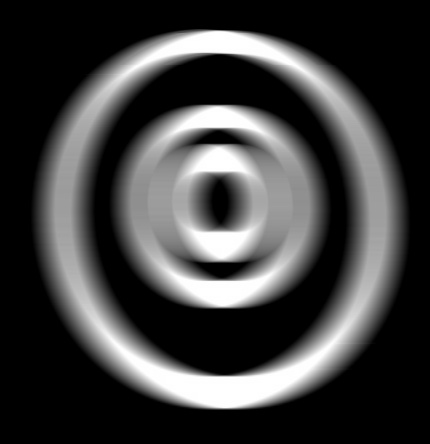
\includegraphics[width=.22\linewidth]{concentric_01_5_blurred_180.jpg}  
  
\includegraphics[width=.22\linewidth]{concentric_01_5_blurred_45.jpg}
  
\includegraphics[width=.22\linewidth]{concentric_01_5_blurred_90.jpg}  
  
\includegraphics[width=.22\linewidth]{concentric_01_5_blurred_135.jpg}
  \caption{Sample images used to create training data for the fiducial pattern
  with binary code ``01''}
\end{figure}

\section{Experimental Validation}
First, we have used synthetic images to test resilience to blur. We have scaled
down ARTag fiducial and our fiducial to size 150x150.  Then, we blurred both
fiducials along all orientations using different scales. Finally, we tried to
detect ARTag in these blurred images using ALVAR library\cite{alvar} and our fiducial
using algorithm given in previous section.

%\begin{tabular}

%\end{tabular}
Our system has been tested on the image sequences captured from AR Drone
quadcopter. Each image sequence contains frames containing different fiducial
pattern. Sample output for each fiducial pattern is shown in Fig.
\ref{fig:output0} -- Fig. \ref{fig:output3}.

\begin{figure}
\centering
  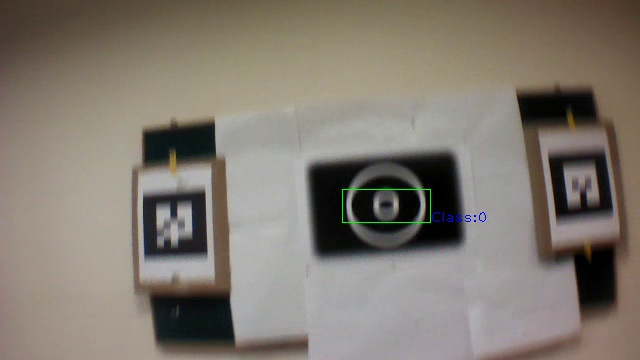
\includegraphics[width=.8\linewidth]{output_00.jpg}
  \caption{Sample output for the fiducial pattern with binary code ``00''}
  \label{fig:output0}
\end{figure}

\begin{figure}
\centering
  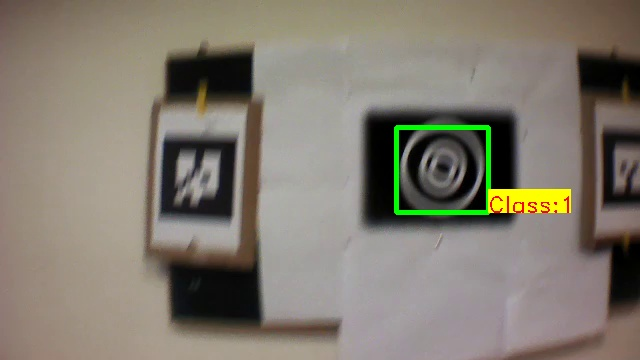
\includegraphics[width=.8\linewidth]{output_01.jpg}
  \caption{Sample output for the fiducial pattern with binary code ``01''}
  \label{fig:output1}
\end{figure}

\begin{figure}
\centering
  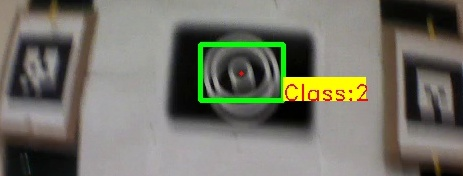
\includegraphics[width=.8\linewidth]{output_10.jpg}
  \caption{Sample output for the fiducial pattern with binary code ``10''}
  \label{fig:output2}
\end{figure}

\begin{figure}
\centering
  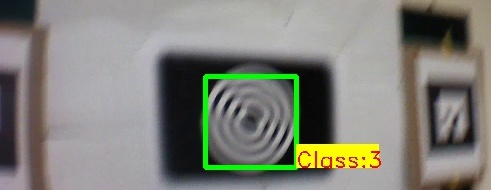
\includegraphics[width=.8\linewidth]{output_11.jpg}
  \caption{Sample output for the fiducial pattern with binary code ``11''}
  \label{fig:output3}
\end{figure}

Our system has also been tested on images containing multiple fiducial patterns
in the same frame. Our algorithm successfully detected all fiducial patterns as
well as correctly classified them as shown in Fig. \ref{fig:output_all}
\begin{figure}
\centering
  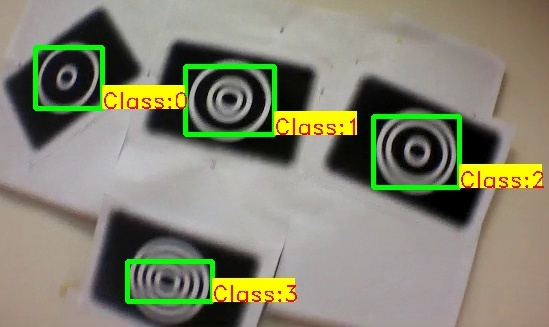
\includegraphics[width=.8\linewidth]{output_all_2.jpg}
  \caption{Sample output containing all two bit binary coded fiducial patterns}
  \label{fig:output_all}
\end{figure}

\subsection{Comparison}
We will compare our results with standard fiducials such as ARTag. Also, we will
compare our results with Blur driven tracker.
\subsubsection{Comparison with ARTag}
\subsubsection{Comparison with Blut} 

\section{Discussion}
\begin{itemize}
\item Processing Time
\item False Positives and False Negatives
\item Pose Estimation
\end{itemize}
\section{Conclusion and Future Work}

\bibliographystyle{splncs}
\bibliography{egbib}

\end{document}

